\documentclass[a4paper]{IEEEtran}

% Packages
\usepackage{siunitx}
\usepackage{tikz}
\usepackage{graphicx}
\usepackage{url}
\usepackage{booktabs}
\usepackage{tabu}
\usepackage{multirow}
\usepackage{listings}
\usepackage{ragged2e}

% Use font weights in text for siunitx
\sisetup{detect-weight=true, detect-family=true}

% Tikz packages
\usetikzlibrary{decorations.pathmorphing, shapes.misc}

% Listings settings
\lstset{
  basicstyle=\scriptsize,
  breaklines=true,
  postbreak=\mbox{$\hookrightarrow$}\space,
  numbers=left,
  numbersep=5pt,
  xleftmargin=2em,
  frame=single
}

% Code and drawings commands
\newcommand{\srbsource}[2]{
\subsubsection{\texttt{\protect\url{#1}}} \mbox{}
\lstinputlisting[language=#2]{../#1}
}

\newcommand{\srbdrawing}[4][0.87]{
\subsubsection{#2}
#4. All dimensions in \SI{}{mm}.
\noindent
\begin{center}
\includegraphics[height=#1\textwidth, angle=90]{#3}
\end{center}
\newpage
}

% NMEA spec environment
\newenvironment{nmeaspec}[1]
{
\newcommand{\field}[2]{\texttt{##1} & ##2 \\}
\vspace{0.2cm}
\noindent\texttt{#1}
\vspace{0.2cm}

\noindent Fields:
\vspace{0.1cm} \\ 
\noindent \vspace{0.2cm}
\begin{tabular}{ll}
}
{
\end{tabular}
}

% Title, author, etc.
\title{\vspace{5.0cm}Autonomous surf life saving device}
\author{\Large Jarod Lam\\ \textit{Supervisor: Matthew Dunbabin}}
\IEEEspecialpapernotice{2018-2019 VRES project at Queensland University of Technology}
\IEEEaftertitletext{\center 13th February 2019 \vspace{1cm}}

\begin{document}

% Title page
\begin{minipage}{\textwidth}
\vfill
\maketitle
\begin{minipage}{\textwidth}
\centering
\includegraphics[width=0.7\textwidth]{boat-overview.jpg}
\end{minipage}
\vfill
\end{minipage}
\clearpage

\begin{abstract}
Life saving services rescue thousands of people every year and are essential to keeping public beaches safe. However, accidents can still happen and life savers are often required to place themselves at risk. This paper describes the design and testing of the Surf Rescue Boat (SRB), a system intended to supplement the work of life saving services at public beaches. The system comprises a semi-autonomous water vehicle (the ``boat"), a communications system, and a computer vision system as an interface for navigation (not developed in this project). The boat uses a life saving rescue board as a base, with two thrusters mounted on the bottom and a waterproof case of electronics on the top. It is intended to roam behind the surf breach and be directed to positions through the communications system from an onshore base station. When a person in distress is identified, the boat is sent by the user to the the GPS coordinates of the person, where the boat provides support while the person is rescued. Over the course of this project, the boat and communications were developed to a stage where they could be tested under controlled conditions in the water; however, time constraints prevented field testing from being completed. Several areas for future development are proposed for this project to move it toward an operational system. The most significant of these proposals is the development of the computer vision component, which will allow GPS positions to be selected from a live onshore camera feed. With more development from its proof of concept stage, the Surf Rescue Boat and similar systems could assist in saving countless lives along public beaches in the future.
\end{abstract}

\setcounter{tocdepth}{2}
\tableofcontents

\section{Introduction}
Surf life savers regularly patrol beaches to help those in danger and are essential to keeping public beaches safe. In Queensland alone, over three thousand are rescued and hundreds are resuscitated by life saving services every year \cite{lifesaving}. However, whilst saving many lives, from 2008-2018, there was an average of 47 drowning deaths per year at Australian beaches--a tragically high number that many organisations are working to reduce \cite{drowning}. In addition, surf conditions can be just as dangerous for the rescuer as they are for the rescuee.

To supplement the activities of surf life savers and other services at public beaches, a system has been proposed that will allow timely help to be given to people in distress while waiting to be rescued. The Surf Rescue Boat (SRB) aims to deliver help quickly and reduce the risk to which life savers are exposed.

The basic concept of the design is a remotely-controlled floating water vehicle that sits behind the surf breach away from the shore at a beach. At most times, the vehicle is idle and remains stationary in the water. When a person in distress is seen, a life saver on the shore can remotely direct the vehicle to the person to support them while they wait for help.

A simple water-based robot such as the one proposed can be constructed relatively cheaply and easily with off-the-shelf components. In the future, systems such as these may become widely available and save the lives of many along coastal beaches.

The Surf Rescue Boat is divided into three main systems, shown in Figure \ref{sysoverview}: the remotely operated water vehicle (the ``boat"), an XBee-based radio communications system between the boat and a base station, and a computer vision-based control system. Out of these, only the vehicle and communications were prototyped in this project; the control system has been developed separately in the past and time constraints prevented it from being implemented.

Design considerations taken into account include cost of construction, parts, and maintenance; usability and user-friendliness; and effectiveness as a water-based vehicle.

This report describes these systems in detail, the design and testing methodology, and avenues that can be explored for future development of the Surf Rescue Boat.

\begin{figure}[h]
\center
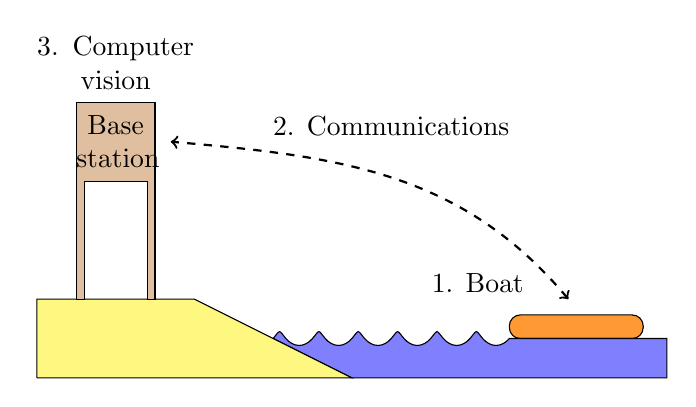
\begin{tikzpicture}

% Boat
\draw [fill=orange!80, rounded corners] (6,0.5) rectangle (7.7,0.8);

% Landscape
\draw [fill=blue!50, decoration={coil, segment length=0.5cm}] (3,0.5) -- (4,0) -- (8,0) -- (8,0.5) -- (6,0.5) decorate { -- (2.5,0.5) };
\draw [fill=yellow!50] (0,0) -- (0,1) -- (2,1) -- (4,0) -- (0,0);

% Tower
\draw [fill=brown!50] (0.5,1) -- (0.5,3.5) -- (1.5,3.5) -- (1.5,1) -- (1.4,1) -- (1.4,2.5) -- (0.6,2.5) -- (0.6,1) -- (0.5,1);

% Comms
\draw [dashed, thick, out=130, in=-5, <->] (6.75,1) to (1.7,3);

% Labels
\draw (1,4) node [text width=2cm, align=center] {3. Computer\\vision};
\draw (4.5,3.2) node {2. Communications};
\draw (5.6,1.2) node {1. Boat};
\draw (1,3) node [text width=1cm, align=center] {Base\\station};

\end{tikzpicture}
\caption{Overview of the Surf Rescue Boat systems on a cross-section of a beach. The boat is behind the surf break and communicates wirelessly with the computer vision base station on a lifeguard tower.}
\label{sysoverview}
\end{figure}

\section{Boat}

The boat comprises mechanical, electrical, and software components. The electronic systems are encased in a box strapped to the topside of a rescue board, while two thrusters are mounted to the underside. Photos of both sides of the boat can be seen in Figure \ref{boatpics}.

\begin{figure}[h!]
\begin{minipage}{0.5\columnwidth}
\includegraphics[width=\textwidth]{boat-top.jpg}
\end{minipage}%
\begin{minipage}{0.5\columnwidth}
\includegraphics[width=\textwidth]{boat-bottom.jpg}
\end{minipage}
\caption{Photos of the top (left) and bottom (right) sides of the boat. The electronics box is strapped to the top and thrusters are mounted to the bottom, with wires connecting around the sides.}
\label{boatpics}
\end{figure}

\subsection{Mechanical}
The remotely operated boat uses a standard rescue board as a base, and houses electronics in a watertight hard plastic case attached to the top. Two thrusters are mounted to the bottom of the rescue board for movement control.

\subsubsection{Chassis}
Rescue board. Chosen for its stability and familiarity in the surf. The standardness and availability of rescue boards is an advantage to encouraging development of such systems. A custom-built chassis may have been designed, but would have taken more time and money. 

\subsubsection{Propellors}
\begin{figure}[h!]
\includegraphics[width=\columnwidth]{motors-mounted.jpg}
\caption{Close-up photo of Blue Robotics T200 thrusters mounted to the underside of the rescue board.}
\label{propmount}
\end{figure}
Two (2) Blue Robotics T200 brushless motor thrusters. A thruster is mounted each to the left and right of the rescue board's middle underside to provide forward and differential steering. Two aluminium mounting plates, one attached to the board with Sikaflex and another that attaches to the thrusters, were designed to distribute force and allow propellors to be detached easily. An image of this setup is shown in Figure \ref{propmount}. Schematics for the mounting plates can be found in Appendix B-B.

\subsubsection{Electronics housing}
Pelican 1120 Case. A laser-cut acrylic frame was made to mount the electronics in the box. Wire glands on the side of the box allow propellor wires to be fed from the thrusters through the box walls.

\subsection{Electronics}
An Arduino Mega 2560 controls the onboard electronics mounted in the case. GPS and IMU modules are used for navigation, and an XBee radio communicates with the base station. Two electronics speed controllers (ESCs) control the two thrusters. A block connection diagram of the electronics setup is shown in Figure \ref{elecdiag}. A CAD rendering of the physical arrangement of the electronics is shown in Figure \ref{elecframe}, and a photo of the electronics assembly is shown in Figure \ref{boathardware}.

\begin{figure}
\center
\pgfdeclarelayer{bg}
\pgfsetlayers{bg,main}
\begin{tikzpicture}

% Arduino
\draw [fill=teal!50] (0,0) rectangle ++(3,3) node [pos=0.5, align=center] (A) {Arduino Mega};

% Batteries
\draw [fill=blue!50] (A)++(-2.5,4.5) rectangle ++(1,-2) node [pos=0.5, rotate=90] (B1) {Battery 1};
\draw [fill=blue!50] (A)++(-1,4.5) rectangle ++(1,-2) node [pos=0.5, rotate=90] (B2) {Battery 2};

% ESCs
\draw [fill=yellow!50] (A)++(-3.5,-4.5) rectangle ++(0.5,2) node [pos=0.5, rotate=90] (E1) {ESC 1};
\draw [fill=yellow!50] (A)++(-2.5,-4.5) rectangle ++(0.5,2) node [pos=0.5, rotate=90] (E2) {ESC 2};

% XBee
\draw [fill=red!50] (A)++(1,4.5) rectangle ++(2,-2) node [pos=0.5] (X) {XBee};

% GPS
\draw [fill=green!80!black!20!white] (A)++(-1.5,-4.5) rectangle ++(2,2) node [pos=0.5] (G) {GPS};

% IMU
\draw [fill=red!50] (A)++(1,-4.5) rectangle ++(2,2) node [pos=0.5] (I) {IMU};

\begin{pgfonlayer}{bg}

% Power lines
\draw [red, thick] (E2)++(0.25,1) -- (B1) node [pos=0.5, rotate=90, above] {11.1V};
\draw [red, thick] (E1)++(0.25,1) -- ++(0,1.25) -- ++(1,0);
\draw [red, thick] (B2) -- ++(0,-1.5) -- ++(-1.5,0);
\draw [red, thick] (A) -- ++(-2,0);

% UART lines
\draw [blue, thick] (G) -- ++(0,2.75) node [pos=0.5, rotate=90, below] {UART};
\draw [blue, thick] (I) -- ++(0,1.5) -- ++(-1.5,0) node [pos=0.5, above] {UART} -- ++(0,1);
\draw [blue, thick] (X) -- ++(0,-1.5) -- ++(-1.5,0) node [pos=0.5, above] {UART} -- ++(0,-1);

% PWM lines
\draw [olive, thick] (E2)++(-0.25,1) -- ++(0,0.3) -- ++(1.5,0) -- ++(0,1);
\draw [olive, thick] (E1)++(-0.25,1) -- ++(0,0.5) -- ++(2.25,0) node[pos=0.45, above] {PWM} -- ++(0,1);

\end{pgfonlayer}

\end{tikzpicture}

\caption{Connection block diagram for onboard electronics.}
\label{elecdiag}
\end{figure}

\begin{figure}
\includegraphics[width=\columnwidth]{assembly.png}
\caption{CAD rendering of internal electronics frame within the Pelican case. Hardware is arranged in three layers and mounted on a clear \SI{3}{mm} frame separated by plastic PCB standoffs. The first layer contains the XBee radio, GPS receiver, and IMU. The second layer contains the two ESCs and the Arduino Mega 2560. The third layer contains the two batteries.}
\label{elecframe}
\end{figure}

\begin{figure}[h!]
\includegraphics[width=\columnwidth]{boat-hardware.jpg}
\caption{Top view of the open Pelican case, showing the assembled electronics mounted on the internal frame. Visible from the top are (left to right, top to bottom): Arduino Mega 2560, XBee radio, GPS receiver, and IMU. The two black wire glands on the outer left side of the case allow thruster wires to pass through the case, which connect to the white screw terminals in the top left.}
\label{boathardware}
\end{figure}

\subsubsection{Microcontroller}
Arduino Mega 2560 with Seeedstudio Grove Mega Shield breakout board. This development board is powerful enough to handle relatively simple communication and processing tasks required to control the boat's sensors and motors. More powerful ARM-based boards such as the Raspberry Pi are less suited to rugged environments, and more difficult to recover from failures. The shield provides robust headers to the UART functions of the Arduino.

\subsubsection{Radio}
Digi XBee Pro S1 on a SparkFun XBee Explorer Regulated. This connects to the Arduino via UART, and creates a wireless serial connection to the base station. The protocol is defined in section 3.

\subsubsection{GPS}
LOCOSYS LS20031 GPS receiver. Sends data to the Arduino via UART using the NMEA 0183 protocol found in section 3. 

\subsubsection{IMU}
Sparkfun SEN-10736 9DOF Razor IMU. Sends data to the Arduino via UART. Currently, only the compass value from the sensor is used. Flashed with the Razor AHRS firmware: \url{https://github.com/Razor-AHRS/razor-9dof-ahrs}

\subsubsection{Motor control}
Two (2) Flycolor Raptor 390 30A ESC. Firmware modified to allow forward and backward thruster movement. Receives PWM control signals from the Arduino with a duty cycle range of \SIrange{1000}{2000}{\micro\second}.

\subsubsection{Battery}
Two (2) Zippy Flightmax Z58003S-30 \SI{5800}{mAh} 3S1P. The two batteries are wired in parallel, with a combined nominal capacity of \SI{11.6}{Ah} and nominal voltage of \SI{11.1}{V}.

\subsection{Software}
The Arduino Mega 2560 is programmed in C++ on top of Arduino default and custom libraries. Efforts were made to keep the code somewhat portable and reusable.

The code is split up into several modules, each handling a section of robot operation. These are described below, and the full code can be found in appendix A.

\subsubsection{\texttt{srb}}
Contains the main loop of the program. Initialises values, classes, etc. Runs update functions for GPS, comms, IMU, nav, and motors. Sends \texttt{SRBSM} message at intervals. An AVR watchdog timer is set to reset the microcontroller at the hardware level if the program hangs and reaches a timeout. 

\subsubsection{\texttt{nmea}}
Defines the \texttt{Nmea} class, which contains functions for constructing and parsing NMEA 0183 sentences. This includes generating and validating checksums, counting the number of fields, appending strings and decimal numbers to a sentence, and parsing a sentence by field. All functions use standard C string libraries, so they do not rely on Arduino libraries and will work outside the Arduino environment. Used by \texttt{SrbGps} and \texttt{SrbComms}.

\subsubsection{\texttt{srb\_stats}}
Defines the \texttt{SrbStats} class, which stores the ID, state, GPS and target location, compass and target heading, and other information related to the current state and navigation of the boat. A pointer to the same instance of this class is passed to most other classes when they are created so that they can read and update this information.

\subsubsection{\texttt{srb\_serial}}
Defines the \texttt{SrbSerial} class, which buffers a hardware serial stream and parses the input when a newline is received. The serial port used is configured when the object is created. This is the base class for \texttt{SrbGps}, \texttt{SrbComms}, and \texttt{SrbImu}.

\subsubsection{\texttt{srb\_gps}}
Defines the \texttt{SrbGps} class, which receives and parses GPS fix data over serial. Latitude, longitude, magnetic variation, and ground speed are parsed from the NMEA \texttt{GPRMC} sentence and stored in the \texttt{SrbStats} object. Conversions are made from knots to metres per second, and degrees/minutes to decimal degrees.

\subsubsection{\texttt{srb\_comms}}
Defines the \texttt{SrbComms} class, which sends and receives messages to and from the base station via the XBee radio. Contains functions for constructing and parsing the proprietary NMEA sentences defined in section 3. Stores information and instructions received in the \texttt{SrbStats} object. Stops the boat if no message is received within a timeout period.

\subsubsection{\texttt{srb\_imu}}
Defines the \texttt{SrbImu} class, which receives data from the Sparkfun IMU over serial. Extracts the compass heading from the serial stream and stores it in the \texttt{SrbStats} object.

\subsubsection{\texttt{srb\_motor}}
Defines the \texttt{SrbMotor} class, which controls motor movement. Receives motor power ranges from -100 to 100 and sets the corresponding PWM duty cycle. Accelerates motors to the desired speed at a safe pace.

\subsubsection{\texttt{srb\_nav}}
Defines the \texttt{SrbNav} class, which controls robot navigation. In manual mode, sets motor speed and orients the boat according to target speed and heading sent from the base station. In auto mode, moves the boat toward a set of coordinates sent from the base station. Motors are controlled with the \texttt{SrbMotor} class.

\section{Communications}
Communications between the SRB and the base station are achieved using XBee radios. By attaching a pair of XBee modules to the base station computer and the on-board Arduino, a virtual serial connection is created between the two devices.

\subsection{Protocol}
NMEA 0183 is a communications specification designed to create a standardised serial interface for GPS devices. Every NMEA `sentence' begins with a \texttt{\$} and ends with \texttt{*CS\textbackslash r\textbackslash n}, where \texttt{CS} is a two-digit hexadecimal checksum of the sentence. Some advantages of using NMEA sentences are that they are standardised, human-readable, robust, and relatively simple to implement. 

A common NMEA sentence type is \texttt{GPRMC}, the GPS recommended minimum. This sentence is used to receive information from the onboard GPS module. \texttt{GPRMC} sentences are specified as follows: \cite{gpsinfo}

\begin{nmeaspec}{\$GPRMC,<Time>,<Status>,<Lat>,<LatDir>,\\<Lon>,<LonDir>,<Speed>,<Angle>,<Date>,\\<MagVar>,<MagDir>*CS}
\field{<Time>}{UTC timestamp in HHmmss format}
\field{<Status>}{Status \texttt{A}=active, \texttt{V}=void}
\field{<Lat>}{Latitude in ddmm.mmm format}
\field{<LatDir>}{\texttt{N} or \texttt{S} hemisphere}
\field{<Lon>}{Longitude in dddmm.mmm format}
\field{<LonDir>}{\texttt{E} or \texttt{W} hemisphere}
\field{<Speed>}{Ground speed in knots}
\field{<Angle>}{Track angle in degrees from north}
\field{<Date>}{Date in DDMMYY format}
\field{<MagVar>}{Magnetic variation magnitude}
\field{<MagDir>}{Magnetic variation direction}
\end{nmeaspec}

A NMEA sentence parser and constructor was written in C++ and Python for the boat and the base station, respectively. Specified below is a set of custom NMEA sentence types that was created for communication between the boat and the base station over the XBee radios.

\subsubsection{\texttt{SRBSM} - Status Message}
The \texttt{SRBSM} sentence is sent periodically by the boat to update the base station with status information.

\begin{nmeaspec}{\$SRBSM,<ID>,<State>,<Lat>,<Lon>,<Speed>,\\<Heading>,<BattV>,<FwdPower>,\\<TgtHeading>*CS}
\field{<ID>}{ID of target SRB}
\field{<State>}{\texttt{0}=disabled, \texttt{1}=manual, \texttt{2}=auto}
\field{<Lat>}{Latitude in decimal degrees}
\field{<Lon>}{Longitude in decimal degrees}
\field{<Speed>}{Speed in metres per second}
\field{<Heading>}{Compass heading in deg CW from N}
\field{<BattV>}{Current battery voltage}
\field{<FwdPower>}{Forward power from -100 to 100}
\field{<TgtLat>}{Target latitude in decimal degrees}
\field{<TgtLon>}{Target longitude in decimal degrees}
\field{<TgtHeading>}{Target heading in deg CW from N}
\end{nmeaspec}

\subsubsection{\texttt{SRBJS} - Joystick}
The \texttt{SRBJS} sentence is sent by the base station for manual control of the boat.

\begin{nmeaspec}{\$SRBJS,<ID>,<FwdPower>,<Angle>*CS}
\field{<ID>}{ID of target SRB}
\field{<FwdPower>}{Forward power from -100 to 100}
\field{<Angle>}{Angle of movement CW from -180 to 180}
\end{nmeaspec}

\subsubsection{\texttt{SRBWP} - Waypoint}
The \texttt{SRBWP} sentence is sent by the base station to autonomously direct the boat to a set of coordinates.

\begin{nmeaspec}{\$SRBJS,<ID>,<TgtLat>,<TgtLon>*CS}
\field{<ID>}{ID of target SRB}
\field{<TgtLat>}{Target latitude in decimal degrees}
\field{<TgtLon>}{Target longitude in decimal degrees}
\end{nmeaspec}

\subsection{Hardware}

\begin{figure}[h!]
\includegraphics[width=\columnwidth]{comms-hardware.jpg}
\caption{Communications hardware connected via USB to the base station (left), with an XBee radio (right) and FTDI232 USB to serial UART converter (middle).}
\label{commshardware}
\end{figure}

The base station uses an XBee S1 radio on a Sparkfun XBee Explorer Regulated to communicate with the boat. An FTDI232 breakout board allows the computer's USB port to interface with the XBee's UART. This system is shown in Figure \ref{commshardware}.

\subsection{Software}

\begin{figure}[h!]
\includegraphics[width=\columnwidth]{srb-base-screenshot.png}
\caption{Screenshot of \texttt{srb-base.py} showing NMEA sentences sent and received over the XBee connection.}
\label{srbbase}
\end{figure}

The Python program \texttt{srb-base.py} was developed to provide a rudimentary graphical interface for the wireless serial connection over XBee. A screenshot of this program is shown in Figure \ref{srbbase} with serial input and output from the communications hardware.

The Tkinter interface was modelled on the Arduino IDE's Serial Monitor, but is designed to send NMEA sentences instead of arbitrary text over the serial connection.

"Naked" messages without a leading \texttt{\$} or trailing \texttt{*CS} have these added when they are sent, making it easy to send valid sentences. Incoming messages are validated to ensure the correct syntax and checksum, and invalid sentences are shown in red. The NMEA sentence handler class, \texttt{Nmea}, is separated into the file \texttt{nmea.py}.

All incoming and outgoing messages are logged to the GUI window, terminal window, and a log file in the working directory. The log file includes a comma-separated timestamp at the beginning of each line, allowing the log data to be processed in a makeshift way as a spreadsheet.

The source code for \texttt{srb-base.py} and \texttt{nmea.py} can be found in Appendix A. However, this code is unstable and should not be used as-is, as it was written for testing purposes only.

\section{Testing}
Testing will be performed on the power consumption of the boat in a lab setting, as well as the forward speed and turning speed of the boat under typical calm conditions.

Time constraints under VRES meant that most testing could not be completed. Field testing is intended to be carried out in the near future.

\subsection{Power consumption}

\subsubsection{Method}
The boat was elevated in midair on two stands and oriented to face 0 degrees North according to the onboard magnetometers. Two multimeters were connected to the battery, one in parallel measuring the voltage under load, and one in series measuring current.

Starting from an idle state, the message
\begin{center}
\texttt{\$SRBJS,0,<FwdPower>,0*<CS>}
\end{center}
was sent from the base station to the boat, with \texttt{<FwdPower>} as the throttle value being tested. Voltage and current values were recorded once they stabilised. Then, the message
\begin{center}
\texttt{\$SRBJS,0,0,0*46}
\end{center}
was sent from the base station to halt the motors. This was repeated for the throttle levels 0 (idle), 20, 40, 60, 80, and 100.

%\subsubsection{Analysis and discussion}
%\begin{table}[h!]
%\begin{tabu} to \columnwidth {X[c]X[c]X[c]}
%\toprule
%\textbf{Throttle (\SI{}{\%})} & \textbf{Voltage (\SI{}{V})}  & \textbf{Current (\SI{}{A})} \\ \midrule
%0 & & \\ \midrule
%20 & & \\ \midrule
%40 & & \\ \midrule
%60 & & \\ \midrule
%80 & & \\ \midrule
%100 & & \\ \midrule
%\end{tabu}
%\caption{Power consumption test results}
%\end{table}

%\begin{table}[h!]
%\begin{tabu} to \columnwidth {X[1.5c]X[c]X[2c]}
%\toprule
%\textbf{Throttle (\SI{}{\%})} & \textbf{Power (\SI{}{W})}  & \textbf{\SI{11.6}{Ah} runtime (\SI{}{min})} \\ \midrule
%0 & & \\ \midrule
%20 & & \\ \midrule
%40 & & \\ \midrule
%60 & & \\ \midrule
%80 & & \\ \midrule
%100 & & \\ \midrule
%\end{tabu}
%\caption{Power consumption analysis}
%\end{table}


\subsection{Forward speed}

\subsubsection{Method}
The boat was placed in the water at a clear, calm location and oriented along the shoreline. A rope was attached to aid retrieval.

Starting from an idle state, the message
\begin{center}
\texttt{\$SRBJS,0,<FwdPower>,0*<CS>}
\end{center}
was sent from the base station to the boat, with \texttt{<FwdPower>} as the throttle value being tested. After the boat travelled roughly 20 metres, the message
\begin{center}
\texttt{\$SRBJS,0,0,0*46}
\end{center}
was sent back from the base station to halt the motors. The boat was moved back to its starting position. This process was repeated twice for each throttle level being tested, and for unloaded and loaded scenarios.

Messages from the boat were captured into a file using \texttt{srb-base.py}. All messages except for \texttt{SRBSM} were removed by running the terminal command:
\begin{center}
\texttt{\$grep "SRBSM" [logfilename] > results.csv}
\end{center}
which saved the results in a \texttt{.csv} file.

%\subsubsection{Analysis and discussion}
%\begin{table}[h!]
%\begin{tabu} to \columnwidth {X[c]X[c]X[c]X[c]X[c]X[c]X[c]}
%\toprule
%\multirow{2}{*}{\textbf{Throttle (\SI{}{\%})}} & \multicolumn{3}{c}{\textbf{Accel time (\SI{}{s})}}  & \multicolumn{3}{c}{\textbf{Max speed (\SI{}{\m\per\s})}} \\
%& 1 & 2 & avg. & 1 & 2 & avg. \\ \midrule
%25 & & \\ \midrule
%50 & & \\ \midrule
%75 & & \\ \midrule
%100 & & \\ \midrule
%\end{tabu}
%\caption{Forward speed test results}
%\end{table}

%\begin{figure}[h!]
%\centering
%\caption{Forward speed vs. time}
%\end{figure}

\subsection{Turning speed}

\subsubsection{Method}
The boat was placed in the water at a clear, calm location and oriented along the shoreline. A rope was attached to aid retrieval.

Starting from an idle state, the message
\begin{center}
\texttt{\$SRBJS,0,<FwdPower>,180*<CS>}
\end{center}
was sent from the base station to the boat, with \texttt{<FwdPower>} as the throttle value being tested. After a few seconds, the message
\begin{center}
\texttt{\$SRBJS,0,0,0*46}
\end{center}
was sent back from the base station to halt the motors. The boat was moved back to its starting position. This process was repeated twice for each throttle level being tested, and for unloaded and loaded scenarios.

Messages from the boat were captured into a file using \texttt{srb-base.py}. All messages except for \texttt{SRBSM} were removed by running the terminal command:
\begin{center}
\texttt{\$grep "SRBSM" [logfilename] > results.csv}
\end{center}
which saved the results in a \texttt{.csv} file.

\section{Future development}
The Surf Rescue Boat system in its current state is only an early prototype. Significantly more prototyping and testing needs to be done before it can be viably used in a real-world scenario. Some important areas to explore that have been identified are listed below.

\subsection{Boat}

\subsubsection{Power measurement}
In testing, external multimeters were used to measure voltage and current consumption of the boat. In the future, the boat would benefit from onboard power measurement hardware to monitor voltage and current usage in real-time. This could be used to automatically shut down or bring ashore the boat when the batteries are low.

\subsubsection{Number of thrusters}
While the two thrusters on the boat are already decently powerful, more thrusters would allow the boat to move faster under load, and reach a distressed person more quickly. Three or more thrusters arranged in different directions would increase manoeuvrability, and possibly enable onmi-directional movement.

\subsubsection{Battery capacity}
According to documentation, the T200 thrusters consume about \SI{15}{A} of current at \SI{12}{V} with full thrust. Therefore, the two \SI{5.8}{Ah} batteries will only last roughly 20 minutes at full thrust. Much larger batteries, possibly in a separate or larger case, are required for the system to be viably used in real conditions.

\subsubsection{Stability structure}
In rough surf conditions, the boat would likely be tipped over by large waves. The structure needs to be modified to lower its centre of gravity below the water, increasing stability and aiding recovery from upside down positions. This could be done by attaching a heavy metal bar on the underside of the boat that extends into the water.

\subsubsection{Wiring}
The internal frame and electronics inside the casing would benefit from better arrangement and accessibility for maintenance. Most of the signal and power wiring could be consolidated onto a PCB which will improve the arrangement and reliability of connections. At the very least, a power switch added to the current design would make testing much easier.

\subsection{Communications}

\subsubsection{Hardware housing}
The communications hardware connected to the base station is a jumble of wires and exposed electronics. Ideally, these should be housed in a small box that could be easily laser-cut or 3D printed to fit. This would also allow an antenna to be mounted for the base station, increasing the range and reliability of the communications.

\subsubsection{Stationary mechanism}
In its current state, the boat turns off its thrusters when idle. This is not ideal because without powered movement, it will quickly be swept away by waves and currents. A mechanism should be added for the boat to maintain its position through powered movement when not moving to a new location.

\subsubsection{Homing mechanism}
A homing mechanism would allow the boat to be easily retrieved by a single command, and autonomously return to the base station when communications are disrupted or the battery is low. 

\subsection{Computer vision}
Computer vision is the third component of the Surf Rescue Boat system, which was not explored in this project. The purpose of this component is to provide an interface for guiding the boat to a desired location in the surf, without knowing coordinates or using manual joystick control.

This is intended to be accomplished with a live camera feed from a tower on the shore, projected onto a computer or tablet screen. By calibrating the camera feed with a set of real-world coordinates, a simple image homography model can be created that translates camera pixel coordinates to GPS coordinates. 

In this system, a user will select the target position of the boat on the screen, and this position will be automatically translated into GPS coordinates and sent to the boat. The goal of this is to allow the boat to be directed to a person in distress quickly and efficiently.

The computer vision section has been previously worked on in the past, separately from this project. These may be integrated in the future.

\section{Conclusion}
The Surf Rescue Boat system aims to supplement the work of life saving services at public beaches, providing a technological solution that increases the efficiency and reduce the risk involved in life saving duties.

Over the course of this project, two main components of the system were developed: the roaming surface ``boat", and the communications system. Significant amounts of hardware and software were created for both components. These were both developed to a testable stage as first prototypes, but time constraints prevented field testing to be carried out before this report was completed.

The system as it currently stands shows potential to be used in surf rescue situations. However, it is very much a proof-of-concept, and significantly more development and testing is required before it can even be tested in the surf. In particular, the computer vision component needs to be added for the SRB to be viably used in real situations.

With further development, the Surf Rescue Boat could be an invaluable tool for helping people in life saving services help those in distress. In the future, similar systems could help save countless lives in the surf along coastal public beaches.
  
\bibliography{bibliography}
\bibliographystyle{IEEEtran}

\clearpage
\appendices

\section{Code}

\subsection{\texttt{srb}}
\srbsource{srb/srb.ino}{C++}
\srbsource{srb/nmea.h}{C++}
\srbsource{srb/nmea.cpp}{C++}
\srbsource{srb/srb_stats.h}{C++}
\srbsource{srb/srb_serial.h}{C++}
\srbsource{srb/srb_serial.cpp}{C++}
\srbsource{srb/srb_gps.h}{C++}
\srbsource{srb/srb_gps.cpp}{C++}
\srbsource{srb/srb_comms.h}{C++}
\srbsource{srb/srb_comms.cpp}{C++}
\srbsource{srb/srb_imu.h}{C++}
\srbsource{srb/srb_imu.cpp}{C++}
\srbsource{srb/srb_motor.h}{C++}
\srbsource{srb/srb_motor.cpp}{C++}
\srbsource{srb/srb_nav.h}{C++}
\srbsource{srb/srb_nav.cpp}{C++}

\subsection{\texttt{srb-base}}
\srbsource{srb-base/srb-base.py}{Python}
\srbsource{srb-base/nmea.py}{Python}

\onecolumn
\section{Drawings}

\subsection{Electronics housing}
\srbdrawing{Top board}{top-board-drawing.pdf}{\SI{3}{mm} clear acrylic}
\srbdrawing{Middle board}{middle-board-drawing.pdf}{\SI{3}{mm} clear acrylic}
\srbdrawing{Bottom board}{bottom-board-drawing.pdf}{\SI{3}{mm} clear acrylic}

\subsection{Motor mount}
\srbdrawing{Motor mount top}{motor-mount-top-drawing.pdf}{\SI{3}{mm} aluminium}
\srbdrawing{Motor mount bottom}{motor-mount-bottom-drawing.pdf}{\SI{8}{mm} aluminium}

\end{document}